\documentclass[tikz]{standalone}
\usepackage{standalone,ctex,bm,siunitx}
% 各卷共用的数学记号。课程专用记号见相应的主入口。
\RequirePackage{amsmath,amssymb,bm,upgreek}

% 数集与函数空间
\newcommand*{\NN}{\mathbb{N}}
\newcommand*{\ZZ}{\mathbb{Z}}
\newcommand*{\QQ}{\mathbb{Q}}
\newcommand*{\RR}{\mathbb{R}}
\newcommand*{\CC}{\mathbb{C}}
\newcommand*{\FF}{\mathbb{F}}
\newcommand*{\cont}{\mathcal{C}}  % 连续函数空间，\cont^k 表示 k 次连续可微
\newcommand*{\poly}{\mathcal{P}}  % \poly_n 中多项式的次数至多为 n

% 微分与常数。文本中的无点 i 和字母下加点另有明确的命令。
\NewCommandCopy{\dotlessi}{\i}
\NewCommandCopy{\dotbelow}{\d}
\renewcommand*{\i}{\mathrm{i}}
\newcommand*{\nd}{\mathrm{d}}
\renewcommand*{\d}{\mathop{}\!\mathrm{d}}
\newcommand*{\e}{\mathop{}\!\mathrm{e}}
\newcommand*{\const}{\mathrm{const}}
\newcommand*{\vd}{\mathop{}\!\delta}  % 变分、依赖过程的热量或功的微元
\newcommand*{\p}{\partial}
\newcommand{\dd}[2][]{\frac{\d^{#1}}{\nd{#2}^{#1}}}
\newcommand{\dv}[3][]{\frac{\d^{#1}#2}{\nd{#3}^{#1}}}
\newcommand{\pp}[2][]{\frac{\p^{#1}}{\p{#2}^{#1}}}
\newcommand{\pv}[3][]{\frac{\p^{#1}#2}{\p{#3}^{#1}}}
\newcommand{\pw}[3]{\frac{\p^2{#1}}{\p{#2}\p{#3}}}

% 函数与算符
\let\Re\relax
\let\Im\relax
\DeclareMathOperator{\Re}{Re}
\DeclareMathOperator{\Im}{Im}
\DeclareMathOperator{\sech}{sech}
\DeclareMathOperator{\csch}{csch}
\DeclareMathOperator{\sinc}{sinc}
\DeclareMathOperator{\sgn}{sgn}
\DeclareMathOperator{\id}{id}
\DeclareMathOperator{\PV}{PV}
\DeclareMathOperator{\FT}{\mathcal{F}}
\DeclareMathOperator{\Beta}{B}
\DeclareMathOperator*{\argmin}{arg\,min}
\DeclareMathOperator*{\argmax}{arg\,max}
\newcommand*{\bigo}{\mathcal{O}}
\newcommand*{\intR}{\int_{-\infty}^\infty}
\newcommand*{\intRplus}{\int_0^\infty}

% 矢量、线性代数与场算符
\newcommand*{\hatbm}[1]{\hat{\bm{#1}}} % 带帽的粗体符号，含义随卷定义
\newcommand*{\dotbm}[1]{\dot{\bm{#1}}}
\newcommand*{\uvec}[1]{\mathop{}\!\hatbm{#1}}  % 系数后自动留薄空；单独取负写 -{\uvec n}
\newcommand*{\grad}{\nabla}
\renewcommand*{\div}{\nabla\cdot}
\newcommand*{\curl}{\nabla\times}
\newcommand*{\laplacian}{\nabla^2}
\DeclareMathOperator{\rank}{rank}
\DeclareMathOperator{\diag}{diag}
\DeclareMathOperator{\tr}{tr}
\DeclareMathOperator{\Span}{span}
\DeclareMathOperator{\nullsp}{N}
\DeclareMathOperator{\colsp}{C}
\newcommand*{\transp}{^\top}
\newcommand*{\conj}{^\ast}
\newcommand*{\adjoint}{^\dagger}
\newcommand*{\inv}{^{-1}}

% 概率、统计与物理量
\renewcommand*{\P}{\operatorname{P}}  % 段落符号 ¶ 可用 \textparagraph
\DeclareMathOperator{\E}{E}
\DeclareMathOperator{\Var}{Var}
\DeclareMathOperator{\BinDist}{Bin}
\DeclareMathOperator{\NormalDist}{N}
\newcommand*{\avg}[1]{\overline{#1}}
\newcommand*{\NA}{N_{\mathrm{A}}}
\newcommand*{\kB}{k_{\mathrm{B}}}
\newcommand*{\muB}{\mu_{\mathrm{B}}}
\newcommand*{\Ek}{E_{\mathrm{k}}}
\newcommand*{\FWHM}{\mathrm{FWHM}}
\newcommand*{\electron}{\mathrm{e}}       % 粒子标签，如 m_\electron
\newcommand*{\proton}{\mathrm{p}}
\newcommand*{\nucleus}{\mathrm{N}}
\newcommand*{\excitedstate}{\mathrm{e}}
\newcommand*{\groundstate}{\mathrm{g}}
\newcommand*{\CM}{\mathrm{CM}}
\newcommand*{\transv}{\mathrm t}  % 横向分量或模式的标签
\newcommand*{\longit}{\mathrm l}  % 纵向分量或模式的标签
\newcommand*{\electric}{\mathrm e}
\newcommand*{\magnetic}{\mathrm m}
\newcommand*{\incident}{\mathrm i}
\newcommand*{\initial}{\mathrm i}
\newcommand*{\final}{\mathrm f}
\newcommand*{\hi}{\mathrm{hi}}
\newcommand*{\lo}{\mathrm{lo}}
\newcommand*{\eff}{\mathrm{eff}}
\newcommand*{\tot}{\mathrm{tot}}

% 括号与 Dirac 记号。显式声明让公式预览也能读到每个尺寸的命令。
\newcommand{\abs}[1]{\lvert#1\rvert}
\newcommand{\bigabs}[1]{\bigl\lvert#1\bigr\rvert}
\newcommand{\Bigabs}[1]{\Bigl\lvert#1\Bigr\rvert}
\newcommand{\biggabs}[1]{\biggl\lvert#1\biggr\rvert}
\newcommand{\Biggabs}[1]{\Biggl\lvert#1\Biggr\rvert}

\newcommand{\norm}[1]{\lVert#1\rVert}
\newcommand{\bignorm}[1]{\bigl\lVert#1\bigr\rVert}
\newcommand{\Bignorm}[1]{\Bigl\lVert#1\Bigr\rVert}
\newcommand{\biggnorm}[1]{\biggl\lVert#1\biggr\rVert}
\newcommand{\Biggnorm}[1]{\Biggl\lVert#1\Biggr\rVert}

\newcommand{\eval}[1]{{#1}\rvert}
\newcommand{\bigeval}[1]{{#1}\bigr\rvert}
\newcommand{\Bigeval}[1]{{#1}\Bigr\rvert}
\newcommand{\biggeval}[1]{{#1}\biggr\rvert}
\newcommand{\Biggeval}[1]{{#1}\Biggr\rvert}

\newcommand{\floor}[1]{\lfloor#1\rfloor}
\newcommand{\bigfloor}[1]{\bigl\lfloor#1\bigr\rfloor}
\newcommand{\Bigfloor}[1]{\Bigl\lfloor#1\Bigr\rfloor}
\newcommand{\biggfloor}[1]{\biggl\lfloor#1\biggr\rfloor}
\newcommand{\Biggfloor}[1]{\Biggl\lfloor#1\Biggr\rfloor}

\newcommand{\ceil}[1]{\lceil#1\rceil}
\newcommand{\bigceil}[1]{\bigl\lceil#1\bigr\rceil}
\newcommand{\Bigceil}[1]{\Bigl\lceil#1\Bigr\rceil}
\newcommand{\biggceil}[1]{\biggl\lceil#1\biggr\rceil}
\newcommand{\Biggceil}[1]{\Biggl\lceil#1\Biggr\rceil}

\newcommand{\ave}[1]{\langle#1\rangle}
\newcommand{\bigave}[1]{\bigl\langle#1\bigr\rangle}
\newcommand{\Bigave}[1]{\Bigl\langle#1\Bigr\rangle}
\newcommand{\biggave}[1]{\biggl\langle#1\biggr\rangle}
\newcommand{\Biggave}[1]{\Biggl\langle#1\Biggr\rangle}

\newcommand{\set}[2]{\{#1\,\vert\,#2\}}
\newcommand{\bigset}[2]{\bigl\{#1\,\big\vert\,#2\bigr\}}
\newcommand{\Bigset}[2]{\Bigl\{#1\,\Big\vert\,#2\Bigr\}}
\newcommand{\biggset}[2]{\biggl\{#1\,\bigg\vert\,#2\biggr\}}
\newcommand{\Biggset}[2]{\Biggl\{#1\,\Bigg\vert\,#2\Biggr\}}

\newcommand{\division}[2]{{#1}/{#2}}
\newcommand{\bigdivision}[2]{{#1}\big/{#2}}
\newcommand{\Bigdivision}[2]{{#1}\Big/{#2}}
\newcommand{\biggdivision}[2]{{#1}\bigg/{#2}}
\newcommand{\Biggdivision}[2]{{#1}\Bigg/{#2}}

\newcommand{\inp}[2]{\langle#1,#2\rangle}
\newcommand{\biginp}[2]{\bigl\langle#1,#2\bigr\rangle}
\newcommand{\Biginp}[2]{\Bigl\langle#1,#2\Bigr\rangle}
\newcommand{\bigginp}[2]{\biggl\langle#1,#2\biggr\rangle}
\newcommand{\Bigginp}[2]{\Biggl\langle#1,#2\Biggr\rangle}

\newcommand{\bra}[1]{\langle#1\rvert}
\newcommand{\bigbra}[1]{\bigl\langle#1\bigr\rvert}
\newcommand{\Bigbra}[1]{\Bigl\langle#1\Bigr\rvert}
\newcommand{\biggbra}[1]{\biggl\langle#1\biggr\rvert}
\newcommand{\Biggbra}[1]{\Biggl\langle#1\Biggr\rvert}

\newcommand{\ket}[1]{\lvert#1\rangle}
\newcommand{\bigket}[1]{\bigl\lvert#1\bigr\rangle}
\newcommand{\Bigket}[1]{\Bigl\lvert#1\Bigr\rangle}
\newcommand{\biggket}[1]{\biggl\lvert#1\biggr\rangle}
\newcommand{\Biggket}[1]{\Biggl\lvert#1\Biggr\rangle}

\newcommand{\braket}[2]{\langle#1\vert#2\rangle}
\newcommand{\bigbraket}[2]{\bigl\langle#1\big\vert#2\bigr\rangle}
\newcommand{\Bigbraket}[2]{\Bigl\langle#1\Big\vert#2\Bigr\rangle}
\newcommand{\biggbraket}[2]{\biggl\langle#1\bigg\vert#2\biggr\rangle}
\newcommand{\Biggbraket}[2]{\Biggl\langle#1\Bigg\vert#2\Biggr\rangle}

\newcommand{\mel}[3]{\langle#1\vert#2\vert#3\rangle}
\newcommand{\bigmel}[3]{\bigl\langle#1\big\vert#2\big\vert#3\bigr\rangle}
\newcommand{\Bigmel}[3]{\Bigl\langle#1\Big\vert#2\Big\vert#3\Bigr\rangle}
\newcommand{\biggmel}[3]{\biggl\langle#1\bigg\vert#2\bigg\vert#3\biggr\rangle}
\newcommand{\Biggmel}[3]{\Biggl\langle#1\Bigg\vert#2\Bigg\vert#3\Biggr\rangle}

\newcommand{\ketbra}[2]{\lvert#1\rangle\langle#2\rvert}
\newcommand{\bigketbra}[2]{\bigl\lvert#1\bigr\rangle\bigl\langle#2\bigr\rvert}
\newcommand{\Bigketbra}[2]{\Bigl\lvert#1\Bigr\rangle\Bigl\langle#2\Bigr\rvert}
\newcommand{\biggketbra}[2]{\biggl\lvert#1\biggr\rangle\biggl\langle#2\biggr\rvert}
\newcommand{\Biggketbra}[2]{\Biggl\lvert#1\Biggr\rangle\Biggl\langle#2\Biggr\rvert}

% 兼容旧版笔记中的内积与外积命令。
\let\brkt\braket
\let\bigbrkt\bigbraket
\let\Bigbrkt\Bigbraket
\let\biggbrkt\biggbraket
\let\Biggbrkt\Biggbraket
\let\ktbr\ketbra
\let\bigktbr\bigketbra
\let\Bigktbr\Bigketbra
\let\biggktbr\biggketbra
\let\Biggktbr\Biggketbra

\newcommand{\bigp}[1]{\bigl(#1\bigr)}
\newcommand{\Bigp}[1]{\Bigl(#1\Bigr)}
\newcommand{\biggp}[1]{\biggl(#1\biggr)}
\newcommand{\Biggp}[1]{\Biggl(#1\Biggr)}

\newcommand{\bigb}[1]{\bigl[#1\bigr]}
\newcommand{\Bigb}[1]{\Bigl[#1\Bigr]}
\newcommand{\biggb}[1]{\biggl[#1\biggr]}
\newcommand{\Biggb}[1]{\Biggl[#1\Biggr]}

\newcommand{\bigB}[1]{\bigl\{#1\bigr\}}
\newcommand{\BigB}[1]{\Bigl\{#1\Bigr\}}
\newcommand{\biggB}[1]{\biggl\{#1\biggr\}}
\newcommand{\BiggB}[1]{\Biggl\{#1\Biggr\}}

% 公式排版
% 方程组的内容是一个 aligned 块，左花括号随整组方程的高度伸展。
\newcommand{\eqnset}[1]{\left\{#1\right.}
\newcommand{\fracdisp}[2]{\frac{\displaystyle #1}{\displaystyle #2}}
\newcommand*{\vs}{\mathord{\text{–}}}
\newcommand*{\otherwise}{\text{otherwise}}
\newcommand*{\qqquad}{\qquad\quad}
\newcommand*{\qqqquad}{\qquad\qquad}

\renewcommand*{\le}{\leqslant}
\renewcommand*{\leq}{\leqslant}
\renewcommand*{\ge}{\geqslant}
\renewcommand*{\geq}{\geqslant}

% 正文与图册共同使用的核素、稳定性、参考系和截面记号
\newcommand*{\nuc}[1]{\mathrm{#1}}
\NewDocumentCommand{\nuclide}{o m m}{{^{#2}\IfValueT{#1}{_{#1}}\nuc{#3}}}
\newcommand*{\stable}{\text{ (stable)}}
\newcommand*{\LAB}{\mathrm L}
\newcommand*{\scattered}{\mathrm{sc}}
\newcommand*{\reactionlabel}{\mathrm r}

\usetikzlibrary{angles,calc,circuits.ee.IEC,quotes,shapes}

\begin{document}

% Nuclear physics and detectors
\begingroup
\tikzset{>=latex}

\newcommand{\xOy}[4]{
	\draw[thick, <->](0, #4)node[left]{$#3$}--(0, 0)node[shift={(-135:7pt)}]{$O$}--(#2, 0)node[right]{$#1$}
}

\sisetup{uncertainty-mode = separate}

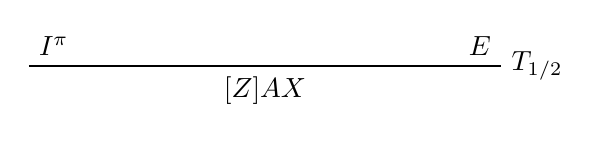
\begin{tikzpicture}
	\draw[thick](0, 0)node[above right]{$I^\pi$}--(6, 0)node[midway, below]{$\nuclide[Z]{A}{X}$}node[above left]{$E$}node[right]{$T_{1/2}$};
    \label{energy-state}
\end{tikzpicture}

\documentclass[tikz,border=2pt]{standalone}
\usepackage{ctex}

\begin{document}
% 按原图“图 1.19 考虑自旋–轨道耦合后的核子能级”的能级顺序重绘。
\begin{tikzpicture}[
    >=latex, x=1cm, y=.44cm, font=\small,
    splitting/.style={densely dashed, black!58, line width=.4pt},
    level/.style={line width=.7pt},
    count/.style={minimum width=2.35em, inner sep=1pt},
    closed/.style={count, draw, rounded corners=1pt, font=\small\bfseries}
]
    \node at (1.15,29) {振子激发能};
    \node at (3.1,29) {耦合前 $n\ell$};
    \node at (7.05,29) {耦合后 $n\ell_j$};
    \node at (8.95,29) {容量 $2j + 1$};
    \node at (10.75,29) {累计数};
    \draw[->] (-.05,0) -- (-.05,27.9) node[above] {$E$};

    % 左列按振子壳层分组。短括号涵盖同一壳层内所画的轨道。
    \foreach \shell/\height in {0/0,1/2.35,2/5.6,3/10.65,4/16.3,5/22.45,6/27.55}
        \node at (1.15,\height) {$\shell\hbar\omega$};
    \foreach \low/\high in {5.15/6.05,9.8/11.5,14.35/18.25,20.15/24.75}
        \draw (2.37,\low) -- (2.23,\low) -- (2.23,\high) -- (2.37,\high);

    \foreach \orbital/\height in {
        1s/0, 1p/2.35, 1d/5.15, 2s/6.05, 1f/9.8, 2p/11.5,
        1g/14.35, 2d/16.85, 3s/18.25, 1h/20.15, 2f/22.65,
        3p/24.75, 1i/27.55}
    {
        \node at (2.95,\height) {$\mathrm{\orbital}$};
        \draw[level] (3.35,\height) -- (4.05,\height) coordinate (parent-\orbital);
    }

    % 依能量递增列出：轨道、2j、图上高度、累计粒子数、闭壳层标记。
    \foreach \orbital/\twoj/\height/\total/\style in {
        1s/1/0/2/closed,
        1p/3/1.85/6/count,    1p/1/2.85/8/closed,
        1d/5/4.7/14/count,    2s/1/5.7/16/count,    1d/3/6.7/20/closed,
        1f/7/8.55/28/closed,
        2p/3/10.4/32/count,   1f/5/11.4/38/count,   2p/1/12.4/40/count,
        1g/9/13.4/50/closed,
        1g/7/15.25/58/count,  2d/5/16.25/64/count,  2d/3/17.25/68/count,
        3s/1/18.25/70/count,  1h/11/19.25/82/closed,
        1h/9/21.1/92/count,   2f/7/22.1/100/count,  2f/5/23.1/106/count,
        3p/3/24.1/110/count,  3p/1/25.1/112/count,  1i/13/26.1/126/closed}
    {
        \draw[splitting] (parent-\orbital) -- (5.5,\height);
        \draw[level] (5.5,\height) -- (6.48,\height);
        \node[anchor=west] at (6.52,\height) {$\mathrm{\orbital}_{\twoj/2}$};
        \node at (8.95,\height) {\the\numexpr\twoj+1\relax};
        \node[\style] at (10.75,\height) {\total};
    }
    \label{spin-orbit-splitting}
\end{tikzpicture}
\end{document}


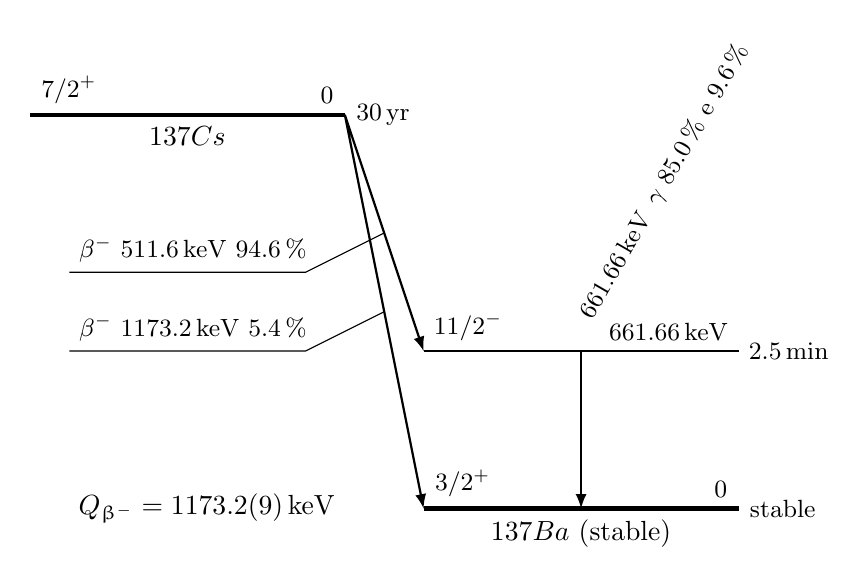
\begin{tikzpicture}
    \draw[ultra thick](-4, 5)node[above right]{\small$7/2^+$}--(0, 5)node[midway, below]{$\nuclide{137}{Cs}$}node[above left]{\small 0}node[right]{\small\qty{30}{yr}};
    \draw[thick, latex-latex](1, 2)--(0, 5)--(1, 0);%node[midway, right]{\qty{94.4}{\percent}}node[midway, left]{\qty{5.6}{\percent}};
    \draw(.5, 3.5)--(-.5, 3)--(-3.5, 3)node[above right]{\small$\beta^-$ \qty{511.6}{keV} \qty{94.6}{\percent}};
    \draw(.5, 2.5)--(-.5, 2)--(-3.5, 2)node[above right]{\small$\beta^-$ \qty{1173.2}{keV} \qty{5.4}{\percent}};
    \draw[thick](1, 2)node[above right]{\small$11/2^-$}--(5, 2)node[above left]{\small \qty{661.66}{keV}}node[right]{\small$\qty{2.5}{min}$};
    \draw[ultra thick](1, 0)node[above right]{\small$3/2^+$}--(5, 0)node[midway, below]{$\nuclide{137}{Ba}\stable$}node[above left]{\small 0}node[right]{\small stable};
    \draw[thick, latex-](3, 0)--(3, 2)node[right, yshift=9pt, rotate=60]{\small \qty{661.66}{keV}\enspace$\gamma$ \qty{85.0}{\percent} e \qty{9.6}{\percent}};%node[midway, right]{\small \qty{661.66}{keV}};
    \node[left]{$Q_{\upbeta^-} = \qty{1173.2+-0.9}{keV}$};
    \label{cesium-decay}
\end{tikzpicture}

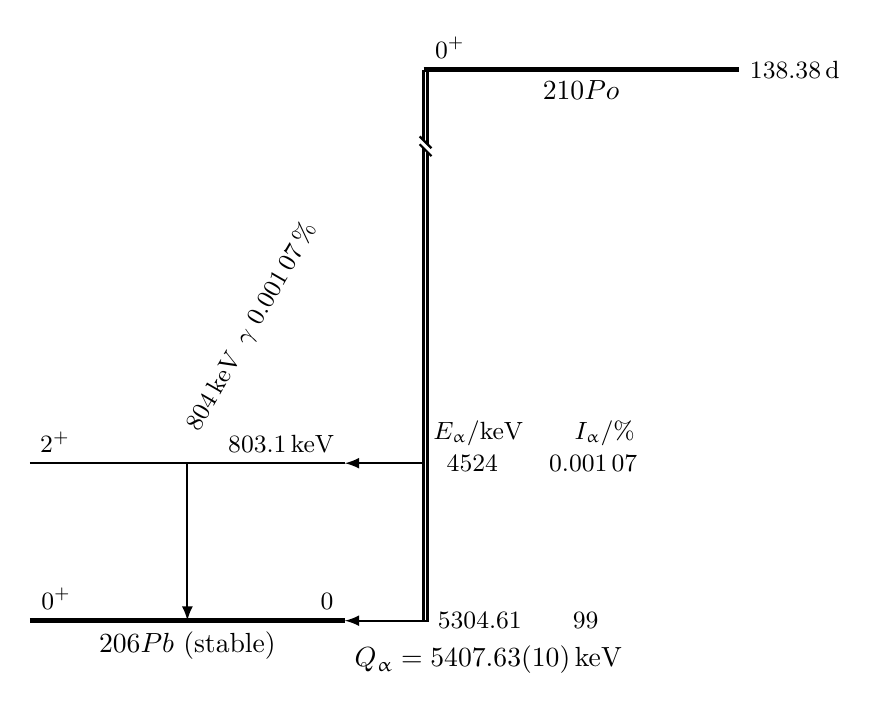
\begin{tikzpicture}
    \node[right]at(4, -.5){$Q_\upalpha = \qty{5407.63+-0.10}{keV}$};
    \draw[ultra thick](0, 0)node[above right]{\small $0^+$}--(4, 0)node[midway, below]{$\nuclide{206}{Pb}\stable$}node[above left]{\small 0};
    \draw[thick](0, 2)node[above right]{\small $2^+$}--(4, 2)node[above left]{\small \qty{803.1}{keV}};
    \draw[thick, latex-](2, 0)--(2, 2)node[right, yshift=9pt, rotate=60]{\small \qty{804}{keV}\enspace$\gamma$ \qty{0.00107}{\percent}};
    \draw[thick, latex-](4, 2)--(5, 2)node[right]{\small\enspace\num{4524}\qquad\num{0.00107}};
    \node[above right]at(5, 2.1){\small$E_\upalpha/\unit{keV}\qquad I_\upalpha/\unit{\percent}$};
    \draw[thick](5, 0)--(5, 6);
    \draw[thick, latex-](4, 0)--(5.05, 0)node[right]{\small\num{5304.61}\qquad 99}--(5.05, 5.95);
    \draw[thick](4.95, 6.05)--(5.1, 5.9);
    \draw[thick](4.95, 6.15)--(5.1, 6);
    \draw[thick](5, 6.1)--(5, 7);
    \draw[thick](5.05, 6.05)--(5.05, 7);
    \draw[ultra thick](5, 7)node[above right]{\small $0^+$}--(9, 7)node[midway, below]{$\nuclide{210}{Po}$}node[right]{\small\qty{138.38}{d}};
    \label{alpha-decay}
\end{tikzpicture}

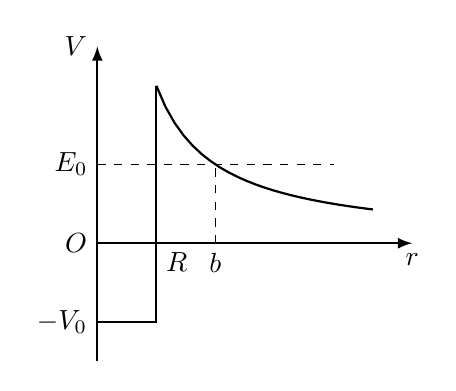
\begin{tikzpicture}
    \draw[thick, -latex](0, -1.5)--(0, 2.5)node[left]{$V$};
    \draw[thick, -latex](0, 0)node[left]{$O$}--(4, 0)node[below]{$r$};
    \draw[dashed](0, 1)node[left]{$E_0$}--(3, 1);
    \draw[thick](0, -1)node[left]{$-V_0$}--(.75, -1)--(.75, 2);
    \draw[dashed](1.5, 0)node[below]{$b$}--(1.5, 1);
    \node[below right]at(.75, 0){$R$};
    \draw[thick, domain=.75:3.5]plot(\x, {1.5/\x});
    \label{coulomb-barrier}
\end{tikzpicture}

\begin{tikzpicture}
    \draw[ultra thick](0, 4)node[above right]{\small$1^+$}--(4, 4)node[midway, below]{$\nuclide{64}{Cu}$}node[right]{\small\qty{12.70}{h}};
    \draw[ultra thick](-4, 0)node[above right]{\small$0^+$}--(-1, 0)node[midway, below]{$\nuclide{64}{Ni}$(稳定)}node[above left]{\small0};
    \draw[thick](-4, 3)node[above right]{$2^+$}--(-1, 3)node[above left]{\small\qty{1345.8}{keV}};
    \draw[ultra thick](5, 2.5)node[above right]{\small$0^+$}--(7, 2.5)node[midway, below]{$\nuclide{64}{Zn}$(稳定)};
    \draw[thick, -latex](4, 4)--(5, 2.5);
    \draw[thick, -latex](0, 4)--(-1, 3);
    \draw[thick, -latex](0, 4)--(-1, 0);
    \draw[thick, -latex](0, 4)--(0, 2)--(-1, 0);
    \draw[thick, latex-](-2.8, 0)--(-2.8, 3)node[right, yshift=9pt, rotate=60]{\small\qty{1345.77}{keV}\enspace$\gamma$ \qty{0.48}{\percent}};
    \draw(4.5, 3.25)--(4, 2.8)--(.5, 2.8)node[above right]{\small$\beta^-$\enspace\qty{578.2}{keV} \qty{37.1}{\percent}}node[below right]{\small $Q_{\upbeta^-} = \qty{578.2+-1.5}{keV}$};
    \draw(-.5, 3.5)--(.5, 1.65)node[above right]{\small EC$_1$}--(4, 1.65)node[above left]{\small \qty{0.48}{\percent}};
    \draw(-.5, 2)--(.5, 1)node[above right]{\small EC$_2$}--(4, 1)node[above left]{\small \qty{44.5}{\percent}};
    \draw(-.5, 1)--(.5, .35)node[above right]{\small$\beta^+$\enspace\qty{652.9}{keV}\enspace\,\qty{17.9}{\percent}}node[below right]{\small$Q_{\mathrm{EC}} = \qty{1674.9+-0.8}{keV}$}--(4, .35);
    \label{copper-decay}
\end{tikzpicture}

\begin{tikzpicture}
    \xOy{p_\upbeta}{4.5}{I(p_\upbeta)}{3};
    \draw[thick, domain=0:4, samples=100]plot(\x, {(2-sqrt(\x^2+9)+3)^2*\x^2/3})node[below]{$p_{\upbeta\max{}}$};
    \draw[dashed](0, 0)parabola(1.5, 3);
    \draw[dashed](4, 0)parabola(3.1, 2.7648);
    \label{beta-phase-space}
\end{tikzpicture}

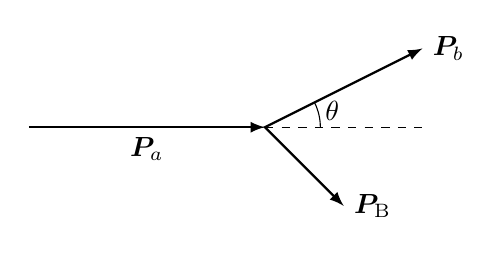
\begin{tikzpicture}
    \coordinate(o)at(0, 0);
    \coordinate(b)at(2, 1);
    \coordinate(c)at(2, 0);
    \coordinate(B)at(1, -1);
    \draw[thick, -latex](-3, 0)--(o)node[midway, below]{$\bm P_a$};
    \draw[thick, latex-latex](B)node[right]{$\bm P_{\nuc B}$}--(o)--(b)node[right]{$\bm P_b$};
    \draw[dashed](o)--(c);
    \pic["$\theta$", draw, angle eccentricity=1.25, angle radius=20]{angle=c--o--b};
    \label{reaction-momentum}
\end{tikzpicture}

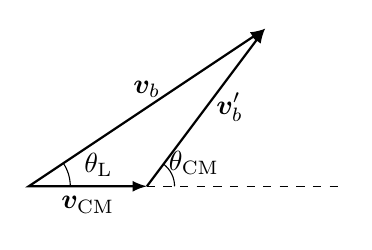
\begin{tikzpicture}
    \coordinate(A)at(0, 0);
    \coordinate(C)at(1.5, 0);
    \coordinate(b)at(3, 2);
    \coordinate(f)at(4, 0);
    % \coordinate(a)at(-1, 0);
    \draw[dashed](C)--(f);
    \draw[thick, -latex](C)--(b)node[midway, right]{$\bm v_b'$};
    \draw[thick, latex-latex](C)--(A)node[midway, below]{$\bm v_\CM$}--(b)node[midway, above]{$\bm v_b$};
    \pic["$\theta_\LAB$", draw, angle eccentricity=1.75, angle radius=15]{angle=f--A--b};
    \pic["$\theta_\CM$", draw, angle eccentricity=1.9, angle radius=10]{angle=f--C--b};
    \label{laboratory-velocities}
\end{tikzpicture}

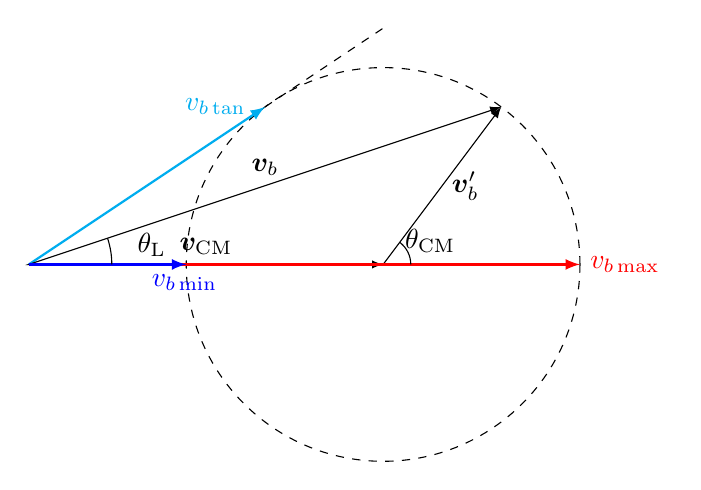
\begin{tikzpicture}
    \coordinate(A)at(-3, 0);
    \coordinate(C)at(1.5, 0);
    \coordinate(b)at(3, 2);
    \coordinate(f)at(4, 0);
    \coordinate(a)at(-1, 0);
    \coordinate(t)at(0, 2);
    \draw[dashed](C)circle(2.5);
    \draw[dashed](t)--(1.5, 3);
    \draw[cyan, thick, -latex](A)--(t)node[left]{$v_{b\tan}~$};
    \draw[-latex](C)--(b)node[midway, right]{$\bm v_b'$};
    \draw[latex-latex](C)--(A)node[midway, above]{$\bm v_\CM$}--(b)node[midway, above]{$\bm v_b$};
    \draw[red, thick, -latex](A)--(f)node[right]{$v_{b\max{}}$};
    \draw[blue, thick, -latex](A)--(a)node[below]{$v_{b\min{}}$};
    \pic["$\theta_\LAB$", draw, angle eccentricity=1.5, angle radius=30]{angle=f--A--b};
    \pic["$\theta_\CM$", draw, angle eccentricity=1.9, angle radius=10]{angle=f--C--b};
    \label{scattering-angles}
\end{tikzpicture}

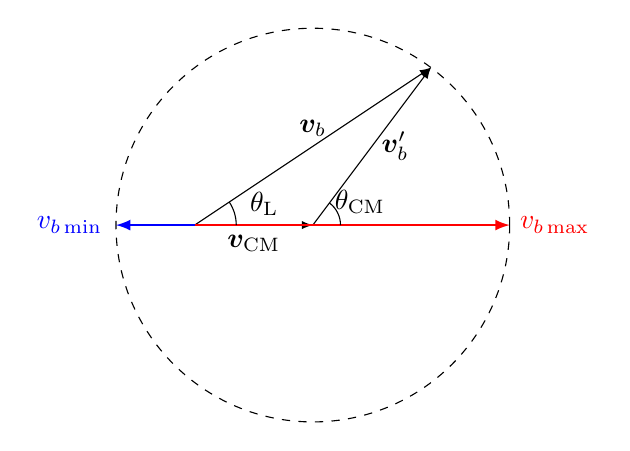
\begin{tikzpicture}
    \coordinate(o)at(0, 0);
    \coordinate(C)at(1.5, 0);
    \coordinate(b)at(3, 2);
    \coordinate(a)at(4, 0);
    \coordinate(d)at(-1, 0);
    \draw[dashed](C)circle(2.5);
    \draw[-latex](C)--(b)node[midway, right]{$\bm v_b'$};
    \draw[latex-latex](C)--(o)node[midway, below]{$\bm v_\CM$}--(b)node[midway, above]{$\bm v_b$};
    \draw[red, thick, -latex](o)--(a)node[right]{$v_{b\max{}}$};
    \draw[blue, thick, -latex](o)--(d)node[left]{$v_{b\min{}}$};
    \pic["$\theta_\LAB$", draw, angle eccentricity=1.75, angle radius=15]{angle=a--o--b};
    \pic["$\theta_\CM$", draw, angle eccentricity=1.9, angle radius=10]{angle=a--C--b};
    \label{scattering-cone}
\end{tikzpicture}

\begin{tikzpicture}
    \draw[thick, domain=0:4, samples=500, fill=gray!50]plot(\x, {2*sqrt(\x)-\x})node[below]{4};
    \xOy{\sigma_{\scattered,0}/(\pi\bar{\lambda}^2)}{4.5}{\sigma_{\reactionlabel,0}/(\pi\bar{\lambda}^2)}{1.5};
    \draw[dashed](0, 1)node[left]{1}--(1, 1)--(1, 0)node[below]{1};
    \label{cross-sections}
\end{tikzpicture}

\begin{tikzpicture}
    \node at(0, 5){直接致电离辐射};
    \node at(7, 5){间接致电离辐射};
    \node(e)at(0,4){快电子};
    \node(X)at(7,4){电磁辐射X,$\gamma$};
    \node(C)at(0,0){重带电粒子};
    \node(n)at(7,0){中子};
    \draw[thick,-latex](X)--(e)node[midway,above]{次级电子}node[midway, below]{光原子反应};
    \draw[thick, -latex](n)--(X)node[midway, right]{原子核(n,$\gamma$)};
    \draw[thick, -latex](n)--(C)node[midway,above]{次级重带电粒子}node[midway, below]{核反应(n,c) (n,f)};
    \draw[thick, -latex](n)--(e)node[midway, sloped, above]{核反应之后的内转换电子};
    \label{ionizing-radiation}
\end{tikzpicture}

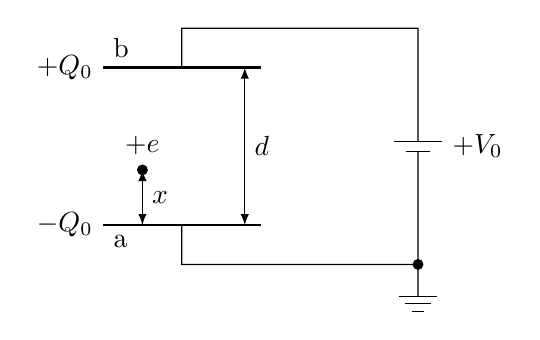
\begin{tikzpicture}[circuit ee IEC]
    \draw [thick] (-4, 2.5) node [left] {$+Q_0$} node [above right] {b} -- (-2, 2.5);
    \draw [thick] (-4, .5) node [left] {$-Q_0$} node [below right] {a} -- (-2, .5);
    \draw [latex-latex] (-2.2, .5) -- (-2.2, 2.5) node [midway, right] {$d$};
    \draw [latex-latex] (-3.5, .5) -- (-3.5, 1.2) node [midway, right] {$x$} node [contact={info={$+e$}}] {};
    \draw (-3, .5) to (-3, 0) to (0, 0) to [ground={at end}] (0, -.5);
    \draw (-3, 2.5) to (-3, 3) to (0, 3) to [battery={info={$+V_0$}}] (0, 0) node [contact] {};
    \label{gas-detector}
\end{tikzpicture}

\begin{tikzpicture}[circuit ee IEC]
    \draw (6, 0) to (0, 0) to [ground={at end}] (0, -.5);
    \draw (2, 3) to (0, 3) to [battery] (0, 0) node [contact] {};
    \draw (2, 0) node [contact] {} to [resistor={info={$R_{\mathrm{L}}$}}] (2, 1.5) to [capacitor={info={$C_1$}}] (2, 3);
    \draw (3.5, 0) node [contact] {} to [capacitor={info={$C'$}}] (3.5, 1.5) node [contact] {};
    \draw (5, 0) node [contact] {} to [resistor={info={$R_{\mathrm{i}}$}}] (5, 1.5) node [contact] {};
    \draw (6, 0) to [capacitor={info={$C_{\mathrm{i}}$}}] (6, 1.5) to (2, 1.5) node [contact] {};
    \draw [dashed] (4.2, -.2) rectangle (6.5, 1.7);
    \node [above] at (5.25, 1.7) {测量仪器};
    \node [right, align=left] at (7, 1.5) {\small$C_1$探测器电容\\$R_{\mathrm{L}}$负载电阻\\$C'$电缆电容等\\$R_{\mathrm{i}}$测量仪器输入电阻\\$C_{\mathrm{i}}$测量仪器输入电容};
    \label{output-circuit}
\end{tikzpicture}

\begin{tikzpicture}
    \xOy t5I4;
    \draw[thick](0, 3)node[left]{$I_1$}--(.5, 3)node[midway, above]{\unit{\micro\second}}--(1, .5)--(3.7, .5)node[midway, above]{\unit{ms}}--(4.2, 0)node[below]{$T^+$};
    \draw[dashed](.5, 3)--(.5, 0)node[below]{$t_1$};
    \draw[dashed](0, .5)node[left]{$I_2$}--(1, .5)--(1, 0)node[below]{$T^-$};
    \draw[dashed](3.7, .5)--(3.7, 0)node[below]{$t_2$};
    \label{ionization-current}
\end{tikzpicture}

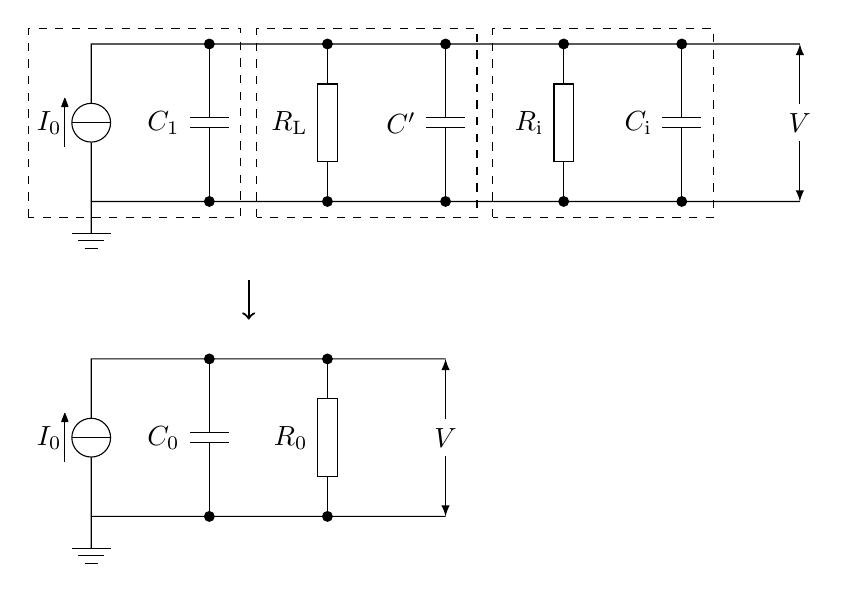
\begin{tikzpicture}[circuit ee IEC]
    \foreach \contact/\x in {1/1.5, 2/3, 3/4.5, 4/6, 5/7.5} {
        \node [contact] (up \contact) at (\x, 2) {};
        \node [contact] (dn \contact) at (\x, 0) {};
    }
    \draw (0, 0) to [current source={direction info={}, info={$I_0$}}] (0, 2) to (9, 2);
    \draw (9, 0) to (0, 0) to [ground={at end}] (0, -.5);
    \draw (dn 1) to [capacitor={info={$C_1$}}] (up 1);
    \draw (dn 2) to [resistor={info={$R_{\mathrm{L}}$}}] (up 2);
    \draw (dn 3) to [capacitor={info={$C'$}}] (up 3);
    \draw (dn 4) to [resistor={info={$R_{\mathrm{i}}$}}] (up 4);
    \draw (dn 5) to [capacitor={info={$C_{\mathrm{i}}$}}] (up 5);
    \draw[latex-latex](9, 0)--(9, 2)node[midway, fill=white]{$V$};
    \draw[dashed](-.8, -.2)rectangle(1.9, 2.2);
    \draw[dashed](2.1, -.2)rectangle(4.9, 2.2);
    \draw[dashed](5.1, -.2)rectangle(7.9, 2.2);
    \draw[thick, ->](2, -1)--(2, -1.5);
    \begin{scope}[yshift=-4cm]
        \foreach \contact/\x in {1/1.5, 2/3} {
            \node [contact] (up \contact) at (\x, 2) {};
            \node [contact] (dn \contact) at (\x, 0) {};
        }
        \draw (0, 0) to [current source={direction info={}, info={$I_0$}}] (0, 2) to (4.5, 2);
        \draw (4.5, 0) to (0, 0) to [ground={at end}] (0, -.5);
        \draw (dn 1) to [capacitor={info={$C_0$}}] (up 1);
        \draw (dn 2) to [resistor={info={$R_0$}}] (up 2);
        \draw[latex-latex](4.5, 0)--(4.5, 2)node[midway, fill=white]{$V$};
    \end{scope}
    \label{chamber-equivalent-circuit}
\end{tikzpicture}

\begin{tikzpicture}[yscale=.8]
    \xOy t{5.5}V{4.2};
    \draw[thick](0, 0)--(1, 2)--(4.2, 3.5);
    \draw[thick, domain=4.2:5]plot(\x, {3.5^((7.2-\x)/3)});
    \draw[dashed](0, 2)node[left]{$Q^-/C_0$}--(1, 2)--(1, 0)node[below]{$T^-$};
    \draw[dashed](0, 3.5)node[left]{$N_0e/C_0$}--(4.2, 3.5)--(4.2, 0)node[below]{$T^+$};
    \label{ion-pulse}
\end{tikzpicture}

\begin{tikzpicture}
    \xOy t4V3;
    \draw[thick](0, 0)--(1, 2);
    \draw[thick, domain=1:3.5]plot(\x, {2^(2-\x)});
    \draw[dashed](0, 2)node[left]{$Q^-/C_0$}--(1, 2)--(1, 0)node[below]{$T^-$};
    \label{electron-pulse}
\end{tikzpicture}

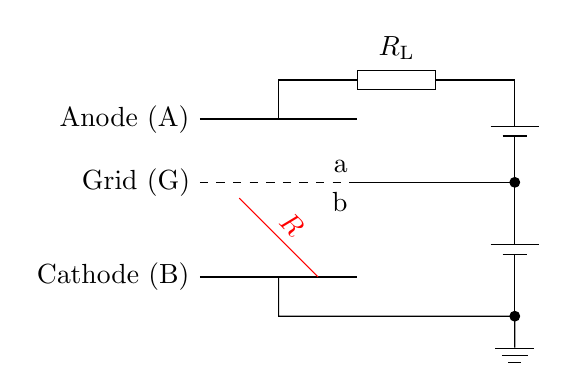
\begin{tikzpicture}[circuit ee IEC]
    \draw [thick] (-4, 2.5) node [left] {Anode (A)} -- (-2, 2.5);
    \draw [thick] (-4, .5) node [left] {Cathode (B)} -- (-2, .5);
    \draw [dashed] (-4, 1.7) node [left] {Grid (G)} -- (-2, 1.7) node [above left] {a} node [below left] {b};
    \draw (-2, 1.7) -- (0, 1.7);
    \draw (-3, .5) to (-3, 0) to (0, 0) to [ground={at end}] (0, -.5);
    \draw (-3, 2.5) to (-3, 3) to [resistor={info={$R_{\mathrm{L}}$}}] (0, 3) to [battery] (0, 1.7) node [contact] {} to [battery] (0, 0) node [contact] {};
    \draw [red] (-3.5, 1.5) -- (-2.5, .5) node [midway, above, sloped] {$R$};
    \label{gridded-chamber}
\end{tikzpicture}

\begin{tikzpicture}
    \xOy {V_0}6h4;
    \draw[thick](2, 2)parabola(0, 0);
    \draw[thick](2, 2)--(4, 2.1);
    \draw[thick](4, 2.1)parabola(5, 3)node[above]{正比区};
    \draw[dashed](0, 2)--(2, 2);
    \draw[dashed](0, 1.8)node[left]{\qty{90}{\percent}}--(1.37, 1.8)--(1.37, 0)node[below]{$V_1$};
    \draw[dashed](4, 2.1)--(4, 0)node[below]{$V_2$};
    \draw[dashed](2.25, 2)--(2.25, 0)node[below]{$V_{\mathrm{work}}$};
    \node[above right]at(0, 3){复合区};
    \node[above]at(2.75, 3){饱和区};
    \label{saturation-curve}
\end{tikzpicture}

\begin{tikzpicture}
    \xOy h6n4;
    \draw[thick, domain=0:1.5]plot(\x, {3*exp(-4*\x*\x)});
    \node[right]at(0, 3){电子学噪声};
    \draw[dashed, domain=.25:1.75]plot(\x, {2*exp(-16*(\x-1)*(\x-1))});
    \node[below]at(1, 0){复合区};
    \draw[thick, domain=-1:1, shift={(3.6, 0)}]plot(\x, {1.2*exp(-6*\x*\x)});
    \draw[thick, domain=-1:1, shift={(4, 0)}]plot(\x, {exp(-4*\x*\x)});
    \draw[thick, domain=-1:1, shift={(4.4, 0)}]plot(\x, {.8*exp(-3*\x*\x)});
    \draw[dashed](3.6, 0)node[below]{$h_1$}--(3.6, 1.5);
    \draw[dashed](4, 0)node[below]{$h_2$}--(4, 1.5);
    \draw[dashed](4.4, 0)node[below]{$h_3$}--(4.4, 1.5);
    \node at(3, -1){(a)};
    \label{pulse-height-spectrum}
\end{tikzpicture}
\begin{tikzpicture}
    \xOy {V_0}4n4;
    \draw[dashed](2, 0)node[below]{$V_1$}--(2, 3);
    \draw[thick](3.5, 1)--(2, 1)node[midway, above]{$h_1$}parabola(1, 0);
    \draw[thick](3.5, 1.75)--(2, 1.75)node[midway, above]{$h_2$}parabola(.75, 0);
    \draw[thick](3.5, 2.5)--(2, 2.5)node[midway, above]{$h_3$}parabola(.5, 0);
    \node at(2, -1){(b)};
    \label{plateau-curve}
\end{tikzpicture}
\endgroup

\begingroup
\standaloneconfig{border=5mm}
% Adapted from Ivan Griffin's Periodic Table of Chemical Elements (2009).
% https://texample.net/periodic-table-of-chemical-elements/ — LPPL 1.3 or later.
\documentclass[tikz,border=5mm]{standalone}
\usetikzlibrary{calc}

\begin{document}
\begingroup
% The atlas uses CTeX's larger type sizes and line spacing. Set the chart's
% type locally so the fixed cells have the same metrics in either document.
\linespread{1}\fontsize{10}{12}\selectfont
% Fixed rows keep long names and configurations within their own cell.
\newcommand{\ElemLabel}[5]{%
  \begin{minipage}[c][2.25cm][s]{2.28cm}
    \centering
    \textbf{#2}\hfill #3\par
    \vfill
    {\fontsize{20.74}{25}\selectfont\bfseries #4\par}
    \vfill
    {\fontsize{9}{11}\selectfont\strut #1\par}
    {\fontsize{9}{11}\selectfont\strut\mbox{#5}\par}
  \end{minipage}%
}

\newcommand{\orbitalS}[1]{s\textsuperscript{#1}}
\newcommand{\orbitalP}[1]{p\textsuperscript{#1}}
\newcommand{\orbitalD}[1]{d\textsuperscript{#1}}
\newcommand{\orbitalF}[1]{f\textsuperscript{#1}}

\newcommand{\ElementEntry}[5][]{\ElemLabel{#1}{#2}{#3}{#4}{#5}}
\newcommand{\TransuraniumEntry}[5][]{\ElemLabel{#1}{#2}{#3}{\textcolor{black!65}{#4}}{#5}}

\begin{tikzpicture}[font=\sffamily]

  % Fill Color Styles
  \tikzstyle{ElementFill} = [fill=yellow!15]
  \tikzstyle{AlkaliMetalFill} = [fill=blue!55]
  \tikzstyle{AlkalineEarthMetalFill} = [fill=blue!40]
  \tikzstyle{MetalFill} = [fill=blue!25]
  \tikzstyle{MetalloidFill} = [fill=orange!40]
  \tikzstyle{NonmetalFill} = [fill=teal!40]
  \tikzstyle{HalogenFill} = [fill=yellow!40]
  \tikzstyle{NobleGasFill} = [fill=green!55]
  \tikzstyle{LanthanideActinideFill} = [fill=red!40]

  % Element Styles
  \tikzstyle{Element} = [ElementFill,
    minimum width=2.5cm, minimum height=2.5cm, node distance=2.75cm]
  \tikzstyle{AlkaliMetal} = [Element, AlkaliMetalFill]
  \tikzstyle{AlkalineEarthMetal} = [Element, AlkalineEarthMetalFill]
  \tikzstyle{Metal} = [Element, MetalFill]
  \tikzstyle{Metalloid} = [Element, MetalloidFill]
  \tikzstyle{Nonmetal} = [Element, NonmetalFill]
  \tikzstyle{Halogen} = [Element, HalogenFill]
  \tikzstyle{NobleGas} = [Element, NobleGasFill]
  \tikzstyle{LanthanideActinide} = [Element, LanthanideActinideFill]
  \tikzstyle{PeriodLabel} = [font={\sffamily\fontsize{17.28}{22}\selectfont}, node distance=2.0cm]
  \tikzstyle{GroupLabel} = [font={\sffamily\fontsize{17.28}{22}\selectfont}, minimum width=2.75cm, node distance=2.0cm]

  % Group 1
  \node[Nonmetal] (H) {\ElementEntry[1\orbitalS1]{1}{1.0079}{H}{Hydrogen}};
  \node[below of=H, AlkaliMetal] (Li) {\ElementEntry[2\orbitalS1]{3}{6.941}{Li}{Lithium}};
  \node[below of=Li, AlkaliMetal] (Na) {\ElementEntry[3\orbitalS1]{11}{22.990}{Na}{Sodium}};
  \node[below of=Na, AlkaliMetal] (K) {\ElementEntry[4\orbitalS1]{19}{39.098}{K}{Potassium}};
  \node[below of=K, AlkaliMetal] (Rb) {\ElementEntry[5\orbitalS1]{37}{85.468}{Rb}{Rubidium}};
  \node[below of=Rb, AlkaliMetal] (Cs) {\ElementEntry[6\orbitalS1]{55}{132.91}{Cs}{Caesium}};
  \node[below of=Cs, AlkaliMetal] (Fr) {\ElementEntry[7\orbitalS1]{87}{(223)}{Fr}{Francium}};

  % Group 2
  \node[right of=Li, AlkalineEarthMetal] (Be) {\ElementEntry[2\orbitalS2]{4}{9.0122}{Be}{Beryllium}};
  \node[below of=Be, AlkalineEarthMetal] (Mg) {\ElementEntry[3\orbitalS2]{12}{24.305}{Mg}{Magnesium}};
  \node[below of=Mg, AlkalineEarthMetal] (Ca) {\ElementEntry[4\orbitalS2]{20}{40.078}{Ca}{Calcium}};
  \node[below of=Ca, AlkalineEarthMetal] (Sr) {\ElementEntry[5\orbitalS2]{38}{87.62}{Sr}{Strontium}};
  \node[below of=Sr, AlkalineEarthMetal] (Ba) {\ElementEntry[6\orbitalS2]{56}{137.33}{Ba}{Barium}};
  \node[below of=Ba, AlkalineEarthMetal] (Ra) {\ElementEntry[7\orbitalS2]{88}{(226)}{Ra}{Radium}};

  % Group 3
  \node[right of=Ca, Metal] (Sc) {\ElementEntry[3\orbitalD14\orbitalS2]{21}{44.956}{Sc}{Scandium}};
  \node[below of=Sc, Metal] (Y) {\ElementEntry[4\orbitalD15\orbitalS2]{39}{88.906}{Y}{Yttrium}};
  \node[below of=Y, LanthanideActinide] (LaLu) {\ElementEntry{57--71}{}{La--Lu}{Lanthanide}};
  \node[below of=LaLu, LanthanideActinide] (AcLr) {\ElementEntry{89--103}{}{Ac--Lr}{Actinide}};

  % Group 4
  \node[right of=Sc, Metal] (Ti) {\ElementEntry[3\orbitalD24\orbitalS2]{22}{47.867}{Ti}{Titanium}};
  \node[below of=Ti, Metal] (Zr) {\ElementEntry[4\orbitalD25\orbitalS2]{40}{91.224}{Zr}{Zirconium}};
  \node[below of=Zr, Metal] (Hf) {\ElementEntry[5\orbitalD26\orbitalS2]{72}{178.49}{Hf}{Hafnium}};
  \node[below of=Hf, Metal] (Rf) {\TransuraniumEntry[(6\orbitalD27\orbitalS2)]{104}{(267)}{Rf}{Rutherfordium}};

  % Group 5
  \node[right of=Ti, Metal] (V) {\ElementEntry[3\orbitalD34\orbitalS2]{23}{50.942}{V}{Vanadium}};
  \node[below of=V, Metal] (Nb) {\ElementEntry[4\orbitalD45\orbitalS1]{41}{92.906}{Nb}{Niobium}};
  \node[below of=Nb, Metal] (Ta) {\ElementEntry[5\orbitalD36\orbitalS2]{73}{180.95}{Ta}{Tantalum}};
  \node[below of=Ta, Metal] (Db) {\TransuraniumEntry[(6\orbitalD37\orbitalS2)]{105}{(268)}{Db}{Dubnium}};

  % Group 6
  \node[right of=V, Metal] (Cr) {\ElementEntry[3\orbitalD54\orbitalS1]{24}{51.996}{Cr}{Chromium}};
  \node[below of=Cr, Metal] (Mo) {\ElementEntry[4\orbitalD55\orbitalS1]{42}{95.94}{Mo}{Molybdenum}};
  \node[below of=Mo, Metal] (W) {\ElementEntry[5\orbitalD46\orbitalS2]{74}{183.84}{W}{Tungsten}};
  \node[below of=W, Metal] (Sg) {\TransuraniumEntry{106}{(269)}{Sg}{Seaborgium}};

  % Group 7
  \node[right of=Cr, Metal] (Mn) {\ElementEntry[3\orbitalD54\orbitalS2]{25}{54.938}{Mn}{Manganese}};
  \node[below of=Mn, Metal] (Tc) {\ElementEntry[4\orbitalD55\orbitalS2]{43}{(98)}{Tc}{Technetium}};
  \node[below of=Tc, Metal] (Re) {\ElementEntry[5\orbitalD56\orbitalS2]{75}{186.21}{Re}{Rhenium}};
  \node[below of=Re, Metal] (Bh) {\TransuraniumEntry{107}{(270)}{Bh}{Bohrium}};

  % Group 8
  \node[right of=Mn, Metal] (Fe) {\ElementEntry[3\orbitalD64\orbitalS2]{26}{55.845}{Fe}{Iron}};
  \node[below of=Fe, Metal] (Ru) {\ElementEntry[4\orbitalD75\orbitalS1]{44}{101.07}{Ru}{Ruthenium}};
  \node[below of=Ru, Metal] (Os) {\ElementEntry[5\orbitalD66\orbitalS2]{76}{190.23}{Os}{Osmium}};
  \node[below of=Os, Metal] (Hs) {\TransuraniumEntry{108}{(277)}{Hs}{Hassium}};

  % Group 9
  \node[right of=Fe, Metal] (Co) {\ElementEntry[3\orbitalD74\orbitalS2]{27}{58.933}{Co}{Cobalt}};
  \node[below of=Co, Metal] (Rh) {\ElementEntry[4\orbitalD85\orbitalS1]{45}{102.91}{Rh}{Rhodium}};
  \node[below of=Rh, Metal] (Ir) {\ElementEntry[5\orbitalD76\orbitalS2]{77}{192.22}{Ir}{Iridium}};
  \node[below of=Ir, Metal] (Mt) {\TransuraniumEntry{109}{(278)}{Mt}{Meitnerium}};

  % Group 10
  \node[right of=Co, Metal] (Ni) {\ElementEntry[3\orbitalD84\orbitalS2]{28}{58.693}{Ni}{Nickel}};
  \node[below of=Ni, Metal] (Pd) {\ElementEntry[4\orbitalD{10}]{46}{106.42}{Pd}{Palladium}};
  \node[below of=Pd, Metal] (Pt) {\ElementEntry[5\orbitalD96\orbitalS1]{78}{195.08}{Pt}{Platinum}};
  \node[below of=Pt, Metal] (Ds) {\TransuraniumEntry{110}{(281)}{Ds}{Darmstadtium}};

  % Group 11
  \node[right of=Ni, Metal] (Cu) {\ElementEntry[3\orbitalD{10}4\orbitalS1]{29}{63.546}{Cu}{Copper}};
  \node[below of=Cu, Metal] (Ag) {\ElementEntry[4\orbitalD{10}5\orbitalS1]{47}{107.87}{Ag}{Silver}};
  \node[below of=Ag, Metal] (Au) {\ElementEntry[5\orbitalD{10}6\orbitalS1]{79}{196.97}{Au}{Gold}};
  \node[below of=Au, Metal] (Rg) {\TransuraniumEntry{111}{(282)}{Rg}{Roentgenium}};

  % Group 12
  \node[right of=Cu, Metal] (Zn) {\ElementEntry[3\orbitalD{10}4\orbitalS2]{30}{65.38}{Zn}{Zinc}};
  \node[below of=Zn, Metal] (Cd) {\ElementEntry[4\orbitalD{10}5\orbitalS2]{48}{112.41}{Cd}{Cadmium}};
  \node[below of=Cd, Metal] (Hg) {\ElementEntry[5\orbitalD{10}6\orbitalS2]{80}{200.59}{Hg}{Mercury}};
  \node[below of=Hg, Metal] (Cn) {\TransuraniumEntry{112}{(285)}{Cn}{Copernicium}};

  % Group 13
  \node[right of=Zn, Metal] (Ga) {\ElementEntry[4\orbitalS24\orbitalP1]{31}{69.723}{Ga}{Gallium}};
  \node[above of=Ga, Metal] (Al) {\ElementEntry[3\orbitalS23\orbitalP1]{13}{26.982}{Al}{Aluminium}};
  \node[above of=Al, Metalloid] (B) {\ElementEntry[2\orbitalS22\orbitalP1]{5}{10.811}{B}{Boron}};
  \node[below of=Ga, Metal] (In) {\ElementEntry[5\orbitalS25\orbitalP1]{49}{114.82}{In}{Indium}};
  \node[below of=In, Metal] (Tl) {\ElementEntry[6\orbitalS26\orbitalP1]{81}{204.38}{Tl}{Thallium}};
  \node[below of=Tl, Metal] (Nh) {\TransuraniumEntry{113}{(286)}{Nh}{Nihonium}};

  % Group 14
  \node[right of=B, Nonmetal] (C) {\ElementEntry[2\orbitalS22\orbitalP2]{6}{12.011}{C}{Carbon}};
  \node[below of=C, Metalloid] (Si) {\ElementEntry[3\orbitalS23\orbitalP2]{14}{28.085}{Si}{Silicon}};
  \node[below of=Si, Metalloid] (Ge) {\ElementEntry[4\orbitalS24\orbitalP2]{32}{72.630}{Ge}{Germanium}};
  \node[below of=Ge, Metal] (Sn) {\ElementEntry[5\orbitalS25\orbitalP2]{50}{118.71}{Sn}{Tin}};
  \node[below of=Sn, Metal] (Pb) {\ElementEntry[6\orbitalS26\orbitalP2]{82}{207.2}{Pb}{Lead}};
  \node[below of=Pb, Metal] (Fl) {\TransuraniumEntry{114}{(289)}{Fl}{Flerovium}};

  % Group 15
  \node[right of=C, Nonmetal] (N) {\ElementEntry[2\orbitalS22\orbitalP3]{7}{14.007}{N}{Nitrogen}};
  \node[below of=N, Nonmetal] (P) {\ElementEntry[3\orbitalS23\orbitalP3]{15}{30.974}{P}{Phosphorus}};
  \node[below of=P, Metalloid] (As) {\ElementEntry[4\orbitalS24\orbitalP3]{33}{74.922}{As}{Arsenic}};
  \node[below of=As, Metalloid] (Sb) {\ElementEntry[5\orbitalS25\orbitalP3]{51}{121.76}{Sb}{Antimony}};
  \node[below of=Sb, Metal] (Bi) {\ElementEntry[6\orbitalS26\orbitalP3]{83}{208.98}{Bi}{Bismuth}};
  \node[below of=Bi, Metal] (Mc) {\TransuraniumEntry{115}{(290)}{Mc}{Moscovium}};

  % Group 16
  \node[right of=N, Nonmetal] (O) {\ElementEntry[2\orbitalS22\orbitalP4]{8}{15.999}{O}{Oxygen}};
  \node[below of=O, Nonmetal] (S) {\ElementEntry[3\orbitalS23\orbitalP4]{16}{32.065}{S}{Sulphur}};
  \node[below of=S, Nonmetal] (Se) {\ElementEntry[4\orbitalS24\orbitalP4]{34}{78.971}{Se}{Selenium}};
  \node[below of=Se, Metalloid] (Te) {\ElementEntry[5\orbitalS25\orbitalP4]{52}{127.60}{Te}{Tellurium}};
  \node[below of=Te, Metalloid] (Po) {\ElementEntry[6\orbitalS26\orbitalP4]{84}{(209)}{Po}{Polonium}};
  \node[below of=Po, Metal] (Lv) {\TransuraniumEntry{116}{(293)}{Lv}{Livermorium}};

  % Group 17
  \node[right of=O, Halogen] (F) {\ElementEntry[2\orbitalS22\orbitalP5]{9}{18.998}{F}{Fluorine}};
  \node[below of=F, Halogen] (Cl) {\ElementEntry[3\orbitalS23\orbitalP5]{17}{35.453}{Cl}{Chlorine}};
  \node[below of=Cl, Halogen] (Br) {\ElementEntry[4\orbitalS24\orbitalP5]{35}{79.904}{Br}{Bromine}};
  \node[below of=Br, Halogen] (I) {\ElementEntry[5\orbitalS25\orbitalP5]{53}{126.90}{I}{Iodine}};
  \node[below of=I, Halogen] (At) {\ElementEntry[6\orbitalS26\orbitalP5]{85}{(210)}{At}{Astatine}};
  \node[below of=At, Halogen] (Ts) {\TransuraniumEntry{117}{(294)}{Ts}{Tennessine}};

  % Group 18
  \node[right of=F, NobleGas] (Ne) {\ElementEntry[2\orbitalS22\orbitalP6]{10}{20.180}{Ne}{Neon}};
  \node[above of=Ne, NobleGas] (He) {\ElementEntry[1\orbitalS2]{2}{4.0026}{He}{Helium}};
  \node[below of=Ne, NobleGas] (Ar) {\ElementEntry[3\orbitalS23\orbitalP6]{18}{39.948}{Ar}{Argon}};
  \node[below of=Ar, NobleGas] (Kr) {\ElementEntry[4\orbitalS24\orbitalP6]{36}{83.798}{Kr}{Krypton}};
  \node[below of=Kr, NobleGas] (Xe) {\ElementEntry[5\orbitalS25\orbitalP6]{54}{131.29}{Xe}{Xenon}};
  \node[below of=Xe, NobleGas] (Rn) {\ElementEntry[6\orbitalS26\orbitalP6]{86}{(222)}{Rn}{Radon}};
  \node[below of=Rn, NobleGas] (Og) {\TransuraniumEntry{118}{(294)}{Og}{Oganesson}};

  % Periods and IUPAC group numbers
  \foreach \period/\element in {1/H,2/Li,3/Na,4/K,5/Rb,6/Cs,7/Fr}
    \node[left of=\element, PeriodLabel] {\period};
  \foreach \group/\element in {1/H,2/Be,3/Sc,4/Ti,5/V,6/Cr,7/Mn,8/Fe,9/Co,
                               10/Ni,11/Cu,12/Zn,13/B,14/C,15/N,16/O,17/F,18/He}
    \node[above of=\element, GroupLabel] {\group};

  % Lanthanide
  \node[below of=Rf, LanthanideActinide, yshift=-1cm] (La) {\ElementEntry[5\orbitalD16\orbitalS2]{57}{138.91}{La}{Lanthanum}};
  \node[right of=La, LanthanideActinide] (Ce) {\ElementEntry[4\orbitalF15\orbitalD16\orbitalS2]{58}{140.12}{Ce}{Cerium}};
  \node[right of=Ce, LanthanideActinide] (Pr) {\ElementEntry[4\orbitalF36\orbitalS2]{59}{140.91}{Pr}{Praseodymium}};
  \node[right of=Pr, LanthanideActinide] (Nd) {\ElementEntry[4\orbitalF46\orbitalS2]{60}{144.24}{Nd}{Neodymium}};
  \node[right of=Nd, LanthanideActinide] (Pm) {\ElementEntry[4\orbitalF56\orbitalS2]{61}{(145)}{Pm}{Promethium}};
  \node[right of=Pm, LanthanideActinide] (Sm) {\ElementEntry[4\orbitalF66\orbitalS2]{62}{150.36}{Sm}{Samarium}};
  \node[right of=Sm, LanthanideActinide] (Eu) {\ElementEntry[4\orbitalF76\orbitalS2]{63}{151.96}{Eu}{Europium}};
  \node[right of=Eu, LanthanideActinide] (Gd) {\ElementEntry[4\orbitalF75\orbitalD16\orbitalS2]{64}{157.25}{Gd}{Gadolinium}};
  \node[right of=Gd, LanthanideActinide] (Tb) {\ElementEntry[4\orbitalF96\orbitalS2]{65}{158.93}{Tb}{Terbium}};
  \node[right of=Tb, LanthanideActinide] (Dy) {\ElementEntry[4\orbitalF{10}6\orbitalS2]{66}{162.50}{Dy}{Dysprosium}};
  \node[right of=Dy, LanthanideActinide] (Ho) {\ElementEntry[4\orbitalF{11}6\orbitalS2]{67}{164.93}{Ho}{Holmium}};
  \node[right of=Ho, LanthanideActinide] (Er) {\ElementEntry[4\orbitalF{12}6\orbitalS2]{68}{167.26}{Er}{Erbium}};
  \node[right of=Er, LanthanideActinide] (Tm) {\ElementEntry[4\orbitalF{13}6\orbitalS2]{69}{168.93}{Tm}{Thulium}};
  \node[right of=Tm, LanthanideActinide] (Yb) {\ElementEntry[4\orbitalF{14}6\orbitalS2]{70}{173.05}{Yb}{Ytterbium}};
  \node[right of=Yb, LanthanideActinide] (Lu) {\ElementEntry[4\orbitalF{14}5\orbitalD16\orbitalS2]{71}{174.97}{Lu}{Lutetium}};

  % Actinide
  \node[below of=La, LanthanideActinide] (Ac) {\ElementEntry[6\orbitalD17\orbitalS2]{89}{(227)}{Ac}{Actinium}};
  \node[right of=Ac, LanthanideActinide] (Th) {\ElementEntry[6\orbitalD27\orbitalS2]{90}{232.04}{Th}{Thorium}};
  \node[right of=Th, LanthanideActinide] (Pa) {\ElementEntry[5\orbitalF26\orbitalD17\orbitalS2]{91}{231.04}{Pa}{Protactinium}};
  \node[right of=Pa, LanthanideActinide] (U) {\ElementEntry[5\orbitalF36\orbitalD17\orbitalS2]{92}{238.03}{U}{Uranium}};
  \node[right of=U, LanthanideActinide] (Np) {\TransuraniumEntry[5\orbitalF46\orbitalD17\orbitalS2]{93}{(237)}{Np}{Neptunium}};
  \node[right of=Np, LanthanideActinide] (Pu) {\TransuraniumEntry[5\orbitalF67\orbitalS2]{94}{(244)}{Pu}{Plutonium}};
  \node[right of=Pu, LanthanideActinide] (Am) {\TransuraniumEntry[5\orbitalF77\orbitalS2]{95}{(243)}{Am}{Americium}};
  \node[right of=Am, LanthanideActinide] (Cm) {\TransuraniumEntry[5\orbitalF76\orbitalD17\orbitalS2]{96}{(247)}{Cm}{Curium}};
  \node[right of=Cm, LanthanideActinide] (Bk) {\TransuraniumEntry[5\orbitalF97\orbitalS2]{97}{(247)}{Bk}{Berkelium}};
  \node[right of=Bk, LanthanideActinide] (Cf) {\TransuraniumEntry[5\orbitalF{10}7\orbitalS2]{98}{(251)}{Cf}{Californium}};
  \node[right of=Cf, LanthanideActinide] (Es) {\TransuraniumEntry[5\orbitalF{11}7\orbitalS2]{99}{(252)}{Es}{Einsteinium}};
  \node[right of=Es, LanthanideActinide] (Fm) {\TransuraniumEntry[5\orbitalF{12}7\orbitalS2]{100}{(257)}{Fm}{Fermium}};
  \node[right of=Fm, LanthanideActinide] (Md) {\TransuraniumEntry[(5\orbitalF{13}7\orbitalS2)]{101}{(258)}{Md}{Mendelevium}};
  \node[right of=Md, LanthanideActinide] (No) {\TransuraniumEntry[(5\orbitalF{14}7\orbitalS2)]{102}{(259)}{No}{Nobelium}};
  \node[right of=No, LanthanideActinide] (Lr) {\TransuraniumEntry[(5\orbitalF{14}7\orbitalS27\orbitalP1)]{103}{(266)}{Lr}{Lawrencium}};

  % Legend
   \fill[AlkaliMetalFill] ($(La.north -| Fr.west) + (0,1em)$)
     rectangle +(1em, 1em) node[right, yshift=-1.2ex]  (AlkaliMetal) {Alkali Metal};
   \fill[AlkalineEarthMetalFill] ($(AlkaliMetal.west) - (1em,2em)$)
     rectangle +(1em, 1em) node[right, yshift=-1.2ex] (AlkalineEarthMetal) {Alkaline Earth Metal};
   \fill[MetalFill] ($(AlkalineEarthMetal.west) - (1em,2em)$)
     rectangle +(1em, 1em) node[right, yshift=-1.2ex] (Metal) {Metal};
   \fill[MetalloidFill] ($(Metal.west) - (1em,2em)$)
     rectangle +(1em, 1em) node[right, yshift=-1.2ex] (Metalloid) {Metalloid};
   \fill[NonmetalFill] ($(Metalloid.west) - (1em,2em)$)
     rectangle +(1em, 1em) node[right, yshift=-1.2ex] (Non-metal) {Non-metal};
   \fill[HalogenFill] ($(Non-metal.west) - (1em,2em)$)
     rectangle +(1em, 1em) node[right, yshift=-1.2ex] (Halogen) {Halogen};
   \fill[NobleGasFill] ($(Halogen.west) - (1em,2em)$)
     rectangle +(1em, 1em) node[right, yshift=-1.2ex] (NobleGas) {Noble Gas};
   \fill[LanthanideActinideFill] ($(NobleGas.west) - (1em,2em)$)
     rectangle +(1em, 1em) node[right, yshift=-1.2ex] (Lanthanide/Actinide) {Lanthanide/Actinide};

  \node at (Ac -| Fr) [draw, Element, fill=white, yshift=-1cm] (legend) {\ElementEntry[configuration]{Z}{\textit{A}\textsubscript{r} or (\textit{A})}{\fontsize{17.28}{22}\selectfont Symbol}{Name}};
  \node[anchor=west, align=left, xshift=3mm] at (legend.east)
    {\textit{Z}:\ 1--92\\\color{black!65}\textit{Z}:\ 93--118 (transuranium)};

  \node at (H -| Fe) [font=\sffamily\fontsize{24.88}{30}\selectfont\bfseries] {Periodic Table of the Elements};

  \label{periodic-table}
\end{tikzpicture}
\endgroup
\end{document}

\endgroup

\begin{tikzpicture}[>=latex,font=\small]
    \label{coincidence-window}
    \fill[teal!12] (1.95,-.16) rectangle (4.05,1.32);
    \foreach \x in {1.95,4.05}
        \draw[gray,dashed] (\x,-.20) -- (\x,1.53);
    \draw[<->] (1.95,1.53) -- node[above] {$2\tau_{\mathrm s}$} (4.05,1.53);
    \draw[->] (0,1) node[left] {通道 1} -- (6.6,1) node[right] {$t$};
    \draw[->] (0,0) node[left] {通道 2} -- (6.6,0) node[right] {$t$};
    \draw[very thick] (3,1) -- ++(0,.31);
    \node[below right,inner sep=2pt] at (3,1) {$t_1$};
    \draw[gray,dotted] (3,.98) -- (3,-.12);
    \draw[very thick] (2.45,0) -- ++(0,.34);
    \draw[very thick] (5.15,0) -- ++(0,.34);
    \node[below] at (2.45,-.17) {计入符合};
    \node[below] at (5.15,-.17) {窗外};
\end{tikzpicture}

\begin{tikzpicture}[>=latex,font=\small,
    electron/.style={->,thick,blue!65!black},
    photon/.style={->,thick,orange!80!black}]
    \label{scintillator-pmt}
    \draw[thick,fill=teal!6] (-2.55,-.80) rectangle (-.62,.80);
    \draw[thick,rounded corners=4pt] (-.62,-.80) rectangle (5.52,.80);
    \draw[->,thick] (-3.73,.28) node[above right] {射线} -- (-1.95,.02);
    \fill (-1.95,.02) circle (1.7pt);
    \foreach \height in {-.46,-.06,.40}
        \draw[photon] (-1.95,.02) -- (-.62,\height);
    \draw[very thick] (-.62,-.57) -- (-.62,.57);
    \draw[electron] (-.60,-.06) to[bend right=9] (1.08,.45);
    \draw[very thick] (.92,.49) -- (1.38,.49);
    \draw[very thick] (2.34,-.49) -- (2.89,-.49);
    \foreach \offset in {0,.16}
        \draw[electron] (1.08+\offset,.45) to[bend left=7] (2.46+\offset,-.44);
    \foreach \offset in {0,.13,.26}
        \draw[electron] (2.46+\offset,-.44) to[bend right=10] (4.49,.09+\offset);
    \draw[very thick] (4.54,-.46) -- (4.54,.52);
    \draw[->] (4.54,-.27) -- (6.18,-.27) node[right] {读出};
    \node[below] at (-1.72,-.80) {闪烁体};
    \node[above] at (-.62,.80) {光阴极};
    \node[above] at (1.14,.82) {打拿极 $D_1$};
    \node[below] at (2.58,-.80) {打拿极 $D_2$};
    \node[above] at (4.54,.80) {阳极};
\end{tikzpicture}

\end{document}
